
\subsection{Ejercicio A}
Realizamos una heurística golosa para resolver el problema. Lo que hace el algoritmo es lo siguiente. Primero toma los datos de entrada del problema, arma la matriz de adyacencia del grafo y además crea un vector de nodos de tamaño $n$ donde cada nodo contiene guardado su número de nodo y el grado que tiene en el grafo. \\ 
Una vez que se procesaron los datos de entrada, se procede a resolver el problema. Para esto, se ordena el arreglo de nodos según sus grados de mayor a menor. Luego, se crea un arreglo de booleanos de tamaño n, donde cada uno está inicializado en $false$. En este arreglo se guarda si el nodo ya fue visitado o no. También se crea un arreglo llamado $cidm$ donde se guardará la solución. \\ 
Por último, se recorre en orden el arreglo de nodos ordenados según su grado. Si un nodo no fue visitado, se agrega el nodo a $cidm$ y luego se recorre su fila en la matriz de adyacencia, marcando como visitados a todos sus adyacentes (ya que queremos que sea dominante y mínimo).
Una vez que se recorre todo el arreglo, ya tenemos el $cidm$, solo resta mostrarlo por pantalla.


\subsection{Ejercicio B}
Calculemos la complejidad del algoritmo. Para esto dividamos el algoritmo en tres etapas, la entrada de datos, la resolución del problema y la salida de datos. \\ 

En la entrada de datos, se crea la matriz de adyacencia, esto tiene costo temporal $\mathcal{O}(m)$, a la vez, se crea el vector de Nodos, con costo $\mathcal{O}(n)$. Por lo tanto, la entrada de datos tiene costo $\mathcal{O}(n + m)$ \\ 

La resolución del problema, comienza ordenando el arreglo de nodos, esto tiene costo  $\mathcal{O}(n*log(n)$. Luego, crea los vectores con costo constante. Por último, recorre todos los nodos ($n$), y por cada nodo, si no fue visitado, lo agrega a la solución con costo constante y se fija en su fila en la matriz de adyacencia quienes son sus vecinos y los marca como visitados, pero notemos que la matriz de adyacencia tiene marcados $2m$ posiciones, por lo tanto, se realizarán a lo sumo $2m$ operaciones en todo el ciclo, que todo el proceso tiene costo $\mathcal{O}(n + 2m) \in \mathcal{O}(n + m)$. \\ 

Por último, se muestra el $cidm$ aproximado por pantalla, para eso se recorre el vector $cidm$ calculado en la resolución, que tiene a lo sumo tamaño $n$, por lo que tiene costo $\mathcal{O}(n)$. \\ 

Por lo tanto, juntando las tres etapas nos queda un costo total de  $\mathcal{O}(n*log(n) + n + m + n) \in \mathcal{O}(n*log(n) + m $ . \\ 

Entonces, la complejidad del algoritmo es de:

$$ \mathcal{O}(n*log(n) + m)$$

\subsection{Ejercicio C}

Veamos un ejemplo de instancias donde la heurística golosa no funciona. Supongamos que tenemos un grafo $G$ con un nodo central $v$ y sean $w_i$ con $1 \leq i \leq k$ sus $k$ vecinos, y supongamos que todo $w_1$ tiene a su vez $k-2$ vecinos de grado 1, llamemoslos $u_{i,j}$ con $1 \leq i \leq k$ y $1 \leq j \leq k-2$. \\ 

\begin{figure}[h]
\begin{center}
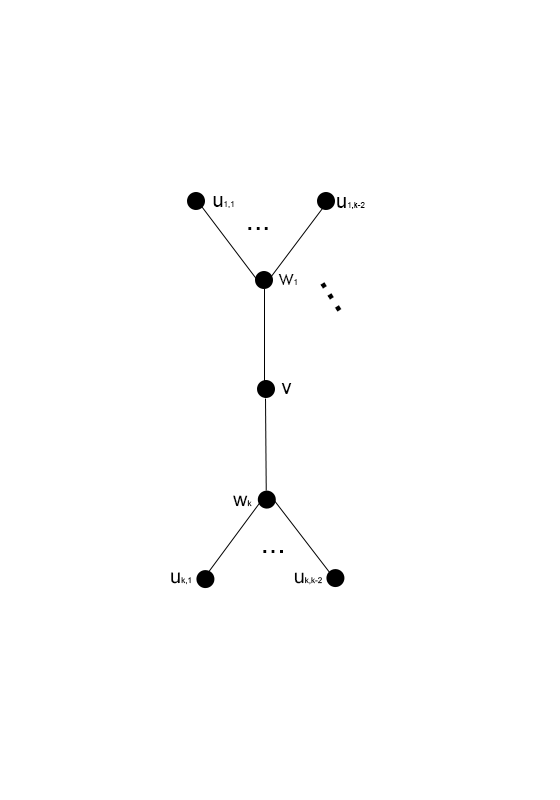
\includegraphics[scale=0.5]{imagenes/grafos-ej3-tp3-1.png}
\end{center}
\end{figure}


 Ahora, al ordenar los nodos según su grado nos quedaría $v$ con $k$ vecinos, luego $w_i$ con $1 \leq i \leq k$, donde cada $w_i$ tiene grado $k-1$, y por último los $k * (k-2)$ nodos $u$ de grado 1. Al correr el algoritmo goloso, este arrojaría un DCIM con cardinalidad $k * (k-2) + 1$ ya que el algoritmo seleccionará a $v$ y a $u_{i,j}$ con $1 \leq i \leq k$ y $1 \leq j \leq k-2$. \\ 

\begin{figure}[h]
\begin{center}
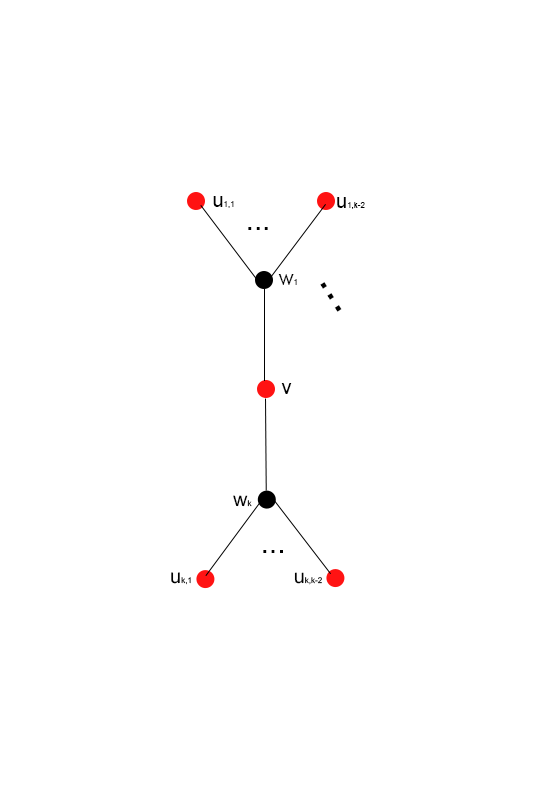
\includegraphics[scale=0.5]{imagenes/grafos-ej3-tp3-2.png}
\end{center}
\end{figure}


 Sin embargo, si seleccionamos a todos los  $w_i$ con $1 \leq i \leq k$, tendríamos un DCIM real con cardinalidad $k$ que es mucho menor que el arrojado por el algoritmo.

\begin{figure}[h]
\begin{center}
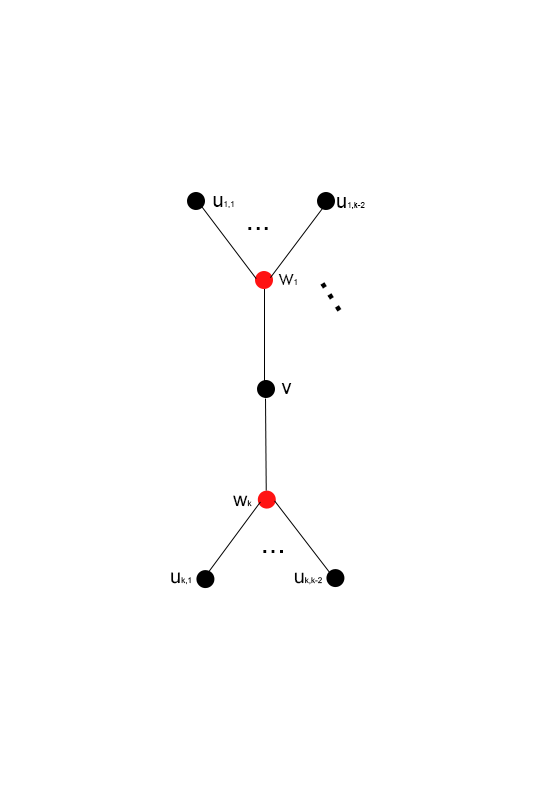
\includegraphics[scale=0.5]{imagenes/grafos-ej3-tp3-3.png}
\end{center}
\end{figure}

Veamos que en este grafo $G=(V,E)$ tenemos $|V| = 1 + k*(k-1)$ nodos y nuestro algoritmo goloso arroja una solución de tamaño $1 + k*(k-2)$ es decir, solo quedan sin seleccionar $k$ nodos. Sin embargo, la solución optima sólo utiliza $k$ nodos. Notemos que el error es cuadrático.


